\documentclass[]{jsarticle}
\usepackage[dvipdfmx]{graphicx}
\usepackage{comment}
\usepackage{listings,jvlisting}
\usepackage{verbatim}
\usepackage{url}
\usepackage[utf8]{inputenc}

\lstset{
  basicstyle={\ttfamily},
  identifierstyle={\small},
  commentstyle={\smallitshape},
  keywordstyle={\small\bfseries},
  ndkeywordstyle={\small},
  stringstyle={\small\ttfamily},
  frame={tb},
  breaklines=true,
  columns=[l]{fullflexible},
  numbers=left,
  xrightmargin=0zw,
  xleftmargin=2zw,
  numberstyle={\scriptsize},
  stepnumber=1,
  numbersep=1zw,
  lineskip=-0.5ex,
}
\renewcommand{\lstlistingname}{ソースコード}
\title{\vspace{-3cm} プログラミング言語実験・C言語 第3回課題レポート}
\author{I類 メディア情報学 \\\textbf{氏名:}LEORA DAVID\\\textbf{学籍番号:}2210745}
\date{2024年05月05日}

\begin{document}
\maketitle

\section*{課題5(コンピュータ大貧民プログラムの実行状況のスクリーンショット)}
大貧民サーバを起動し、大貧民標準クライアント(tndhm\_devkit\_c-20180826.tar.gzに同梱されている方)を5台起動する。
サーバの実行画面(クライアント名が default と表示されている対戦画面)とグラフの画面(棒グラフか線グラフ)の計2画面のスクリーンショットを撮った。\\

\section*{課題5の実行結果}
まず、ターミナルを起動して、「コンピュータ大貧民の実行」ページの通りの手順でサーバを起動した。各フォルダから configure を行い、make を行った。
実行するには、以下のコマンドを実行する。ポート番号は 52745 とした。
\begin{lstlisting}
  $ ./tndhms -p 52745
\end{lstlisting}

また、標準クライアントを起動するには、同じく「コンピュータ大貧民の実行」ページの通りの手順でクライアントを起動した。
実行するには、以下のコマンドを実行する。
\begin{lstlisting}
  $ ./client -p 52745 &
\end{lstlisting}

実行したサーバの実行画面と線グラフの画面のスクリーンショットを以下の図1と図2に示す。
\begin{figure}[h]
  \centering
  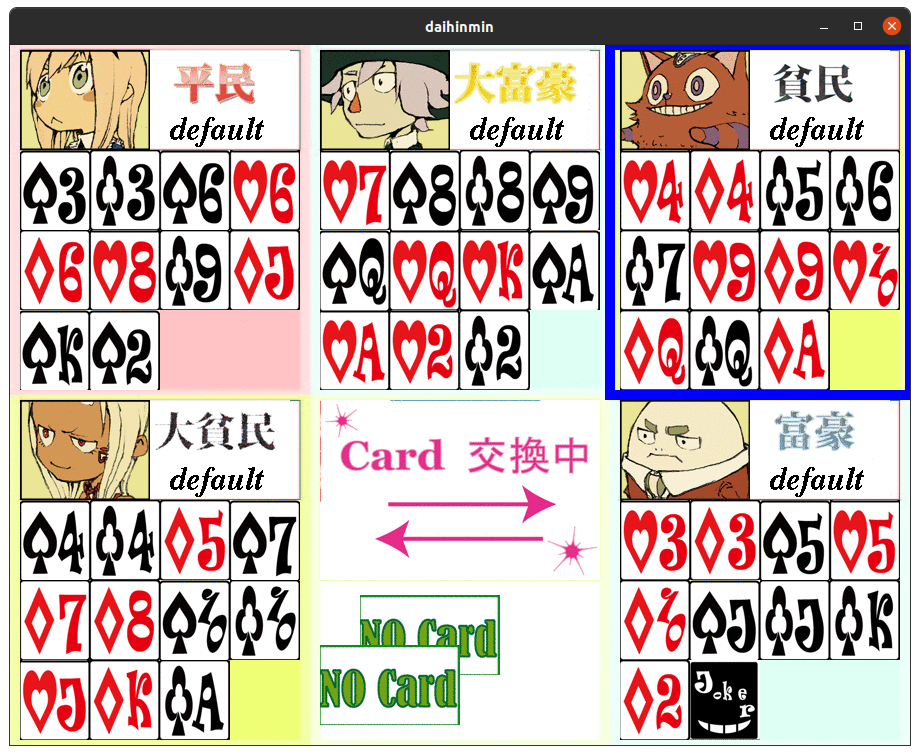
\includegraphics[width=0.5\textwidth]{kadai5/1.png}
  \caption{サーバの実行画面}
\end{figure}

\begin{figure}[h]
  \centering
  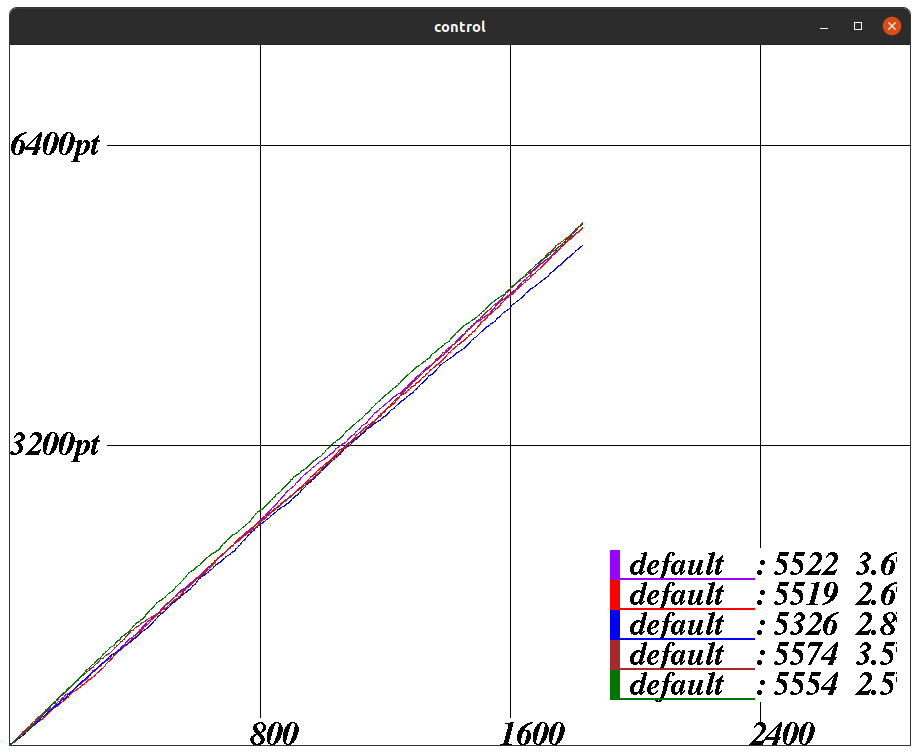
\includegraphics[width=0.5\textwidth]{kadai5/2.png}
  \caption{線グラフの画面}
\end{figure}

\section*{課題6(ペア出し機能の実装)}
コンピュータ大貧民教育用クライアント(tndhmc-0.03.tar.gz)のディレクトリ src にある、select\_cards.c などを改変し、ペア出し機能を実現した。
この課題では、場にカードがない状況で、かつ提出するカードにジョーカーを含まない場合について実装した。
実装が完了したら、大貧民サーバを立ち上げゲームを実行し、ペア出しが行われている様子がわかるスクリーンショットを取得した。
(サーバの実行画面中のクライアントプログラムが Normal と表示されているかを確認した)。\\

実装した「ペア出し機能」のソースコードは以下のソースコード1の通りである。具体的に、daihinmin.c の make\_info\_table 関数と search\_low\_pair 関数を追加した。
make\_info\_table 関数は、自分の手札(my\_cards配列)にあるカードの数を集計し、その情報をinfo\_table配列に格納する。
search\_low\_pair 関数は、手札の中から一番弱いペアを探し、dst\_cards配列に格納する。dst\_cards配列は、提出するカードを格納する配列である。\\

まとめとして、配列は主に以下の目的で使用される。
\begin{itemize}
  \item my\_cards配列:自分の手札のカードを格納する配列である。各要素は特定のカードが手札に存在するかどうかを示す。
  \item info\_table配列:自分の手札のカードの数を集計する配列である。また、info\_table配列は、make\_info\_table 関数で更新される。
  \item dst\_cards配列:提出するカードを格納する配列である。また、dst\_cards配列は、search\_low\_pair 関数で更新される。
  \item select\_cards配列:提出するカードを格納する配列である。
\end{itemize}

また、以下のソースコードによって、search\_low\_pair 関数で、info\_table配列をチェックして最大枚数または一番弱いペア(2枚の場合)を dst\_cards に格納する。
これにより、最大枚数のカードか一番弱いの2枚カードの提出が可能になる。これらの関数と配列の使用により、ペア出し機能が実現されている。


\begin{lstlisting}[caption={daihinmin.c}]
  #include<stdio.h>
  #include<string.h>
  #include<strings.h>
  #include"common.h"
  
  void search_low_card(int out_cards[8][15],int my_cards[8][15],int use_joker_flag){
    /*
      低い方から探して,最初に見つけたカードを一枚out_cardsにのせる。
      use_joker_flagが1のとき,カードが見つからなければ,jokerを一枚out_cardsにのせる。
    */
    int i,j,find_flag=0;
  
    clear_table(out_cards);                  //テーブルをクリア
    for(j=1;j<14&&find_flag==0;j++){        //低い方からさがし
      for(i=0;i<4&&find_flag==0;i++){
        if(my_cards[i][j]==1){              //カードを見つけたら               
          find_flag=1;                      //フラグを立て
          out_cards[i][j]=my_cards[i][j];   //out_cardsにのせ,ループを抜ける。
        }
      }
    }
    if(find_flag==0&&use_joker_flag==1){       //見つからなかったとき
      out_cards[0][14]=2;                  //ジョーカーをのせる
    }
  }
  
  void make_info_table(int info_table[8][15], int my_cards[8][15])
  {
    int i;
  
    clear_table(info_table);
    for(i=1;i<=13;i++){
      info_table[4][i]=my_cards[0][i]+my_cards[1][i]+my_cards[2][i]+my_cards[3][i];
    }
  }
  
  int search_low_pair(int dst_cards[8][15], int info_table[8][15], int my_cards[8][15]){
    int i, j, max_i = 0, max_val = 0;
    clear_table(dst_cards);
    for(i=1; i<=13; i++){
      if(info_table[4][i] > max_val){
        max_val = info_table[4][i];
        max_i = i;
      }
    }
    if(max_val >= 2){
      for(j=0; j<=3; j++) dst_cards[j][max_i] = my_cards[j][max_i];
      return 1;
    }
    else return 0;
  }
\end{lstlisting}

\vspace*{1\baselineskip}
\noindent\textbf{ソースコード1の考察(最大枚数 OR 一番弱いペアの実装)}\\
\indent ソースコード1より、make\_info\_table 関数は、自分の手札にあるカードの数を集計し、その情報をinfo\_table配列に格納する。
具体的に、自分の手札(my\_cards配列)にあるカードの数の情報をinfo\_table配列の4行目(info\_table[4][i])に格納している。
これにより、make\_info\_table 関数は、search\_low\_pair 関数で使用される。dst\_cards 配列をまずクリアし、
for文でinfo\_table配列の4行目(info\_table[4][i])を左から右に順番に探し、\textbf{最大枚数のカード}を探す。最後に、見つかった最大枚数のカードをdst\_cards配列に格納する。\\
もし最大枚数が2の場合、search\_low\_pair 関数は、自分の手札の中から一番弱いペアを探し、dst\_cards 配列に格納する。
また、値が2以上のカードが最後まで見つからない場合、0を返す(0を返すということは、ペアが見つからなかったということである)。\\

次に、select\_cards.c のプログラムの select\_cards\_free の関数に加えました。書いたプログラムをソースコード2に示す。

\begin{lstlisting}[caption={select\_cards.c}]
  #include<stdio.h>
  #include"common.h"
  #include"daihinmin.h"
  #include"select_cards.h"
  
  void select_change_cards(int out_cards[8][15],int my_cards[8][15],int num_of_change){
    /*
     * カード交換時のアルゴリズム
     * 大富豪あるいは富豪が、大貧民あるいは貧民にカードを渡す時のカードを
     * カードテーブルmy_cardsと交換枚数num_of_changeに応じて、
     * 低いほうから選びカードテーブルout_cardsにのせる
    */
    int count=0;
    int one_card[8][15];
    
    clear_table(out_cards);
    while(count<num_of_change){
      search_low_card(one_card,my_cards,0);
      diff_cards(my_cards,one_card);
      or_cards(out_cards,one_card);
      count++;
    }
  }
  
  void select_submit_cards(int out_cards[8][15],int my_cards[8][15], state *field_status){
    int select_cards[8][15];
   
    clear_table(select_cards);
  
    if(field_status->is_rev==0){
      if(field_status->is_no_card==1){                //場にカードが無いとき
        select_cards_free(select_cards, my_cards, field_status);    //通常時の提出用
      }else{
        select_cards_restrict(select_cards,my_cards, field_status);    //通常時の提出用
      }
    }else{
      if(field_status->is_no_card==1){                //場にカードが無いとき
        select_cards_free_rev(select_cards, my_cards, field_status); //革命時の提出用
      }else{
        select_cards_restrict_rev(select_cards, my_cards, field_status); //革命時の提出用
      }
    }
  
    copy_table(out_cards, select_cards);
  }
  
  void select_cards_free(int select_cards[8][15], int my_cards[8][15], state *field_status){
    int info_table[8][15];
  
    make_info_table(info_table, my_cards);
    if(count_cards(select_cards)==0)
      search_low_pair(select_cards, info_table, my_cards); // 手持ちの一番弱いペアを提出する
    if(count_cards(select_cards)==0)
      search_low_card(select_cards,my_cards,0); // 手持ちの一番弱いカードを単騎で提出する
  }
  
  void select_cards_restrict(int select_cards[8][15], int my_cards[8][15], state *field_status){
    int tmp_cards[8][15];
   
    copy_table(tmp_cards, my_cards); 
  
    if(field_status->is_sequence==1){ // 場が階段のとき
      if(field_status->is_lock==1){ // 場が縛られている
  
      }else{ // 場が縛られていない
  
      }
  
    }else if(field_status->quantity > 1){ // 場がペアのとき
      if(field_status->is_lock==1){ // 場が縛られている
  
      }else{ // 場が縛られていない
  
      }
    }else{ // 場が単騎のとき
      if(field_status->is_lock==1){ // 場が縛られている
        remove_suit(tmp_cards, field_status->suit, 1);
        remove_low_card(tmp_cards, field_status->order, 0); 
        search_low_card(select_cards,tmp_cards,1); 
      }else{ // 場が縛られていない
        remove_low_card(tmp_cards, field_status->order, 0); 
        search_low_card(select_cards,tmp_cards,1); 
      }
    }
  }
  
  void select_cards_free_rev(int select_cards[8][15], int my_cards[8][15], state *field_status){
  }
  
  void select_cards_restrict_rev(int select_cards[8][15], int my_cards[8][15], state *field_status){
  }
  
  void operate_my_cards(int my_cards[8][15], state *field_status){
  }
  
  void operate_field_cards(int ba_cards[8][15], state *field_status){
  }
\end{lstlisting}

\vspace*{1\baselineskip}
\noindent\textbf{ソースコード2の考察}\\
\indent ソースコード2より、select\_cards\_free 関数は、場にカードがない状況で、かつ提出するカードにジョーカーを含まない場合について実装した。
具体的に、場にカードがない場合(field\_status-\(>\)is\_no\_card==1)に、select\_cards\_free 関数を呼び出す。
select\_cards\_free 関数は、make\_info\_table 関数を呼び出し、info\_table 配列に自分の手札のカードの数を集計する。
そして、他のプログラム(common.c)から count\_cards 関数を呼び出し、select\_cards 配列のカードの数が0の場合(選択するカードがない場合)に、search\_low\_pair 関数を呼び出す。
search\_low\_pair 関数は、自分の手札の中から\textbf{一番弱いペアではなく、最大枚数}を探し、dst\_cards 配列に格納する。\\
もし、最大枚数が2の場合、search\_low\_pair 関数は、自分の手札の中から一番弱いペアを探し、dst\_cards 配列に格納する。
また、search\_low\_pair 関数でペアが見つからない場合、search\_low\_card 関数を呼び出す。

search\_low\_card 関数は、自分の手札の中から一番弱い単騎カードを探し、dst\_cards 配列に格納する。
最後に、dst\_cards 配列は、提出するカードを格納する配列である。\\

\newpage
\section*{課題6の実行結果}
実装した「ペア出し機能」を確認するために、大貧民サーバを立ち上げ、ゲームを実行した。サーバの実行画面中のクライアントプログラムが Normal と表示されているかを確認した。
ペア出しが行われている様子がわかるスクリーンショットを以下の図3に示す。
\begin{figure}[h]
  \centering
  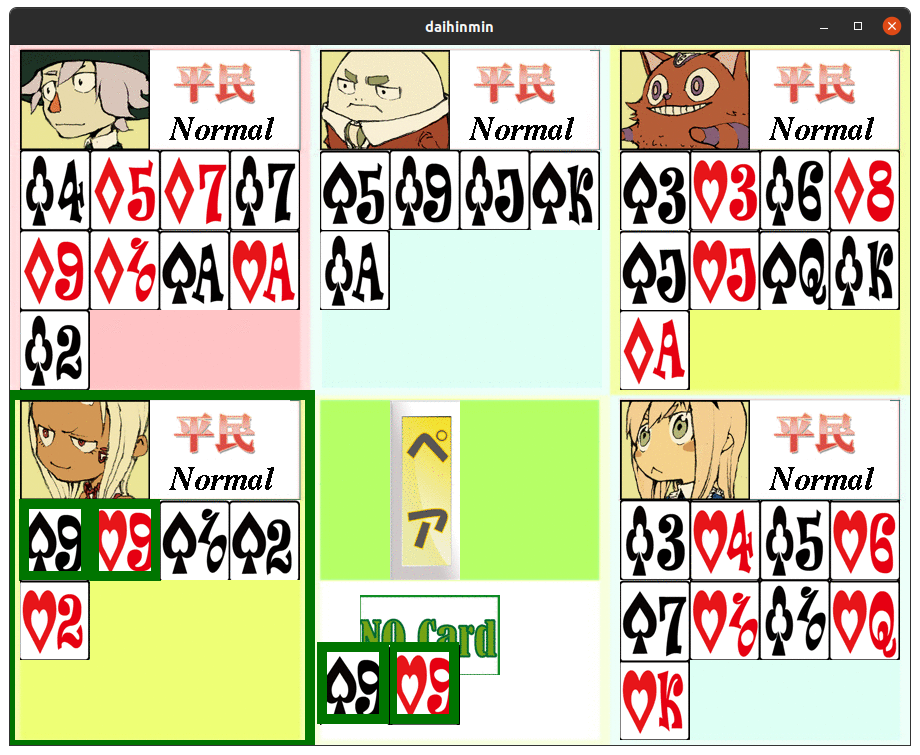
\includegraphics[width=0.5\textwidth]{kadai6/double.png}
  \caption{ペア出し機能の実行画面(カードが2枚ずつ提出されている)}
\end{figure}

また、3枚が提出される場合のスクリーンショットを以下の図4に示す。
\begin{figure}[h]
  \centering
  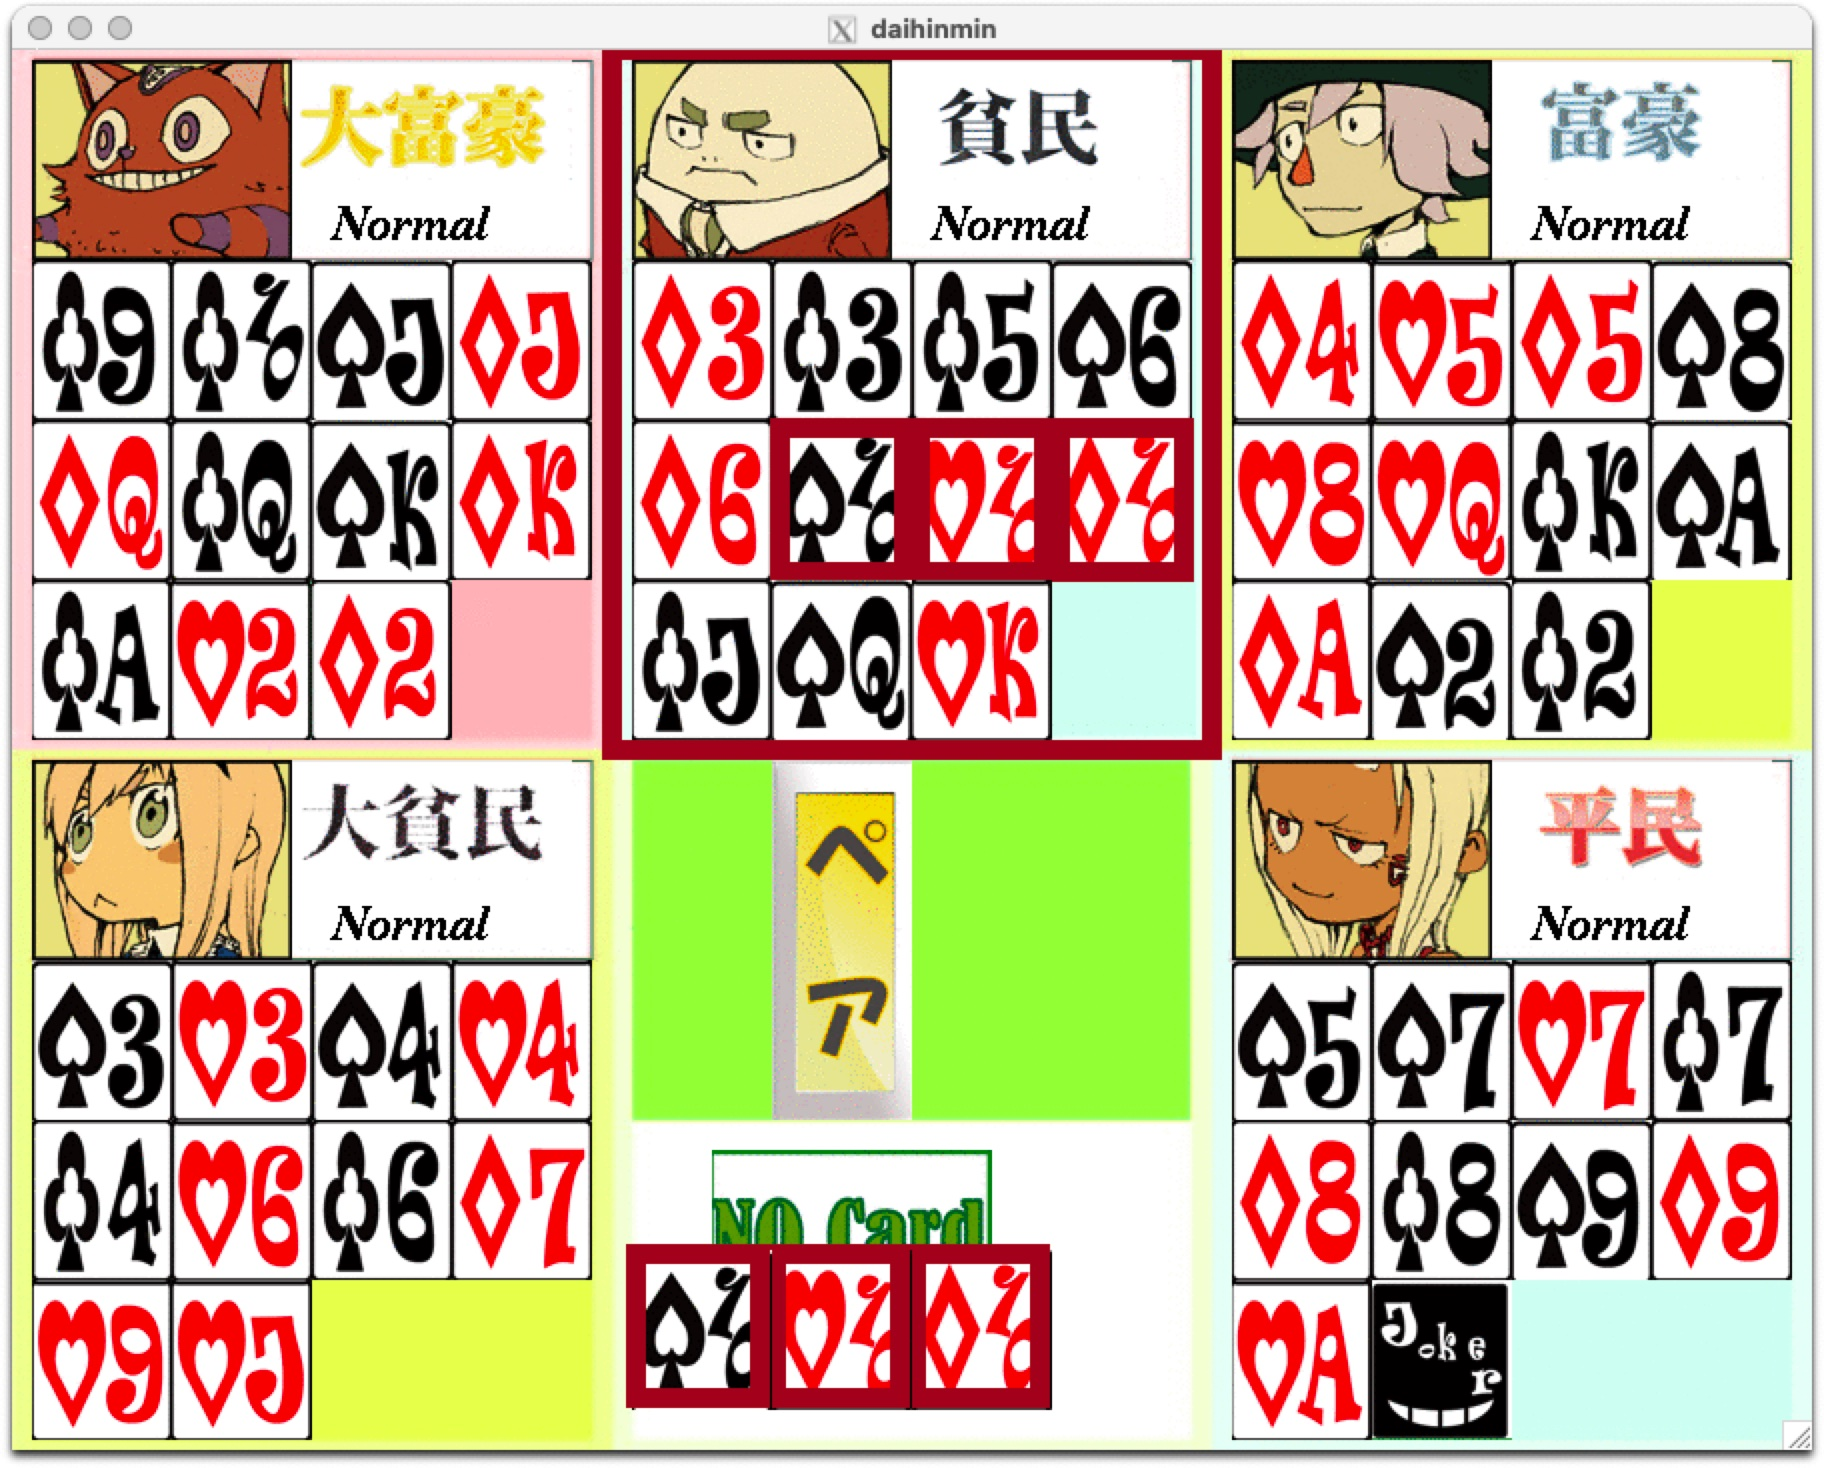
\includegraphics[width=0.5\textwidth]{kadai6/1.jpg}
  \caption{ペア出し機能の実行画面(カードが3枚ずつ提出されている)}
\end{figure}

\newpage
\begin{thebibliography}{99}
  \bibitem{cite1} 第3回 コンピュータ大貧民(大貧民の実行とペア出し機能の実装), \\URL : \url{https://www.ied.inf.uec.ac.jp/text/laboratory/C/third_week/index03.html}
\end{thebibliography}


\end{document}
